%%%%%%%%%%%%%%%%%%%%%%%%%%%%%%%%%%%%%%%%%
% Classicthesis Typographic Thesis
% LaTeX Template
% Version 1.1 (4/8/12)
%
% This template has been downloaded from:
% http://www.LaTeXTemplates.com
%
% Original author:
% André Miede (http://www.miede.de)
%
% License:
% CC BY-NC-SA 3.0 (http://creativecommons.org/licenses/by-nc-sa/3.0/)
%
% General Tips:
% 1) Make sure to edit the classicthesis-config.file
% 2) New enumeration (A., B., C., etc in small caps): \begin{aenumerate} \end{aenumerate}
% 3) For margin notes: \marginpar or \graffito{}
% 4) Do not use bold fonts in this style, it is designed around them
% 5) Use tables as in the examples
% 6) See classicthesis-preamble.sty for useful commands
%
%%%%%%%%%%%%%%%%%%%%%%%%%%%%%%%%%%%%%%%%%

%----------------------------------------------------------------------------------------
%	PACKAGES AND OTHER DOCUMENT CONFIGURATIONS
%----------------------------------------------------------------------------------------

\documentclass[
		twoside,openright,titlepage,numbers=noenddot,headinclude,%1headlines,
                footinclude=true,cleardoublepage=empty,
                BCOR=5mm,paper=a4,fontsize=11pt, % Binding correction, paper type and font size
                english, % Languages
                ]{scrreprt} 
                
% Includes the file which contains all the document configurations and packages - make sure to edit this file
%%%%%%%%%%%%%%%%%%%%%%%%%%%%%%%%%%%%%%%%%
% Thesis Configuration File
%
% The main lines to change in this file are in the DOCUMENT VARIABLES
% section, the rest of the file is for advanced configuration.
%
%%%%%%%%%%%%%%%%%%%%%%%%%%%%%%%%%%%%%%%%%

%----------------------------------------------------------------------------------------
%	DOCUMENT VARIABLES
%	Fill in the lines below to enter your information into the thesis template
%	Each of the commands can be cited anywhere in the thesis
%----------------------------------------------------------------------------------------

% Remove drafting to get rid of the '[ Date - classicthesis version 4.0 ]' text at the bottom of every page
\PassOptionsToPackage{eulerchapternumbers,listings,pdfspacing,subfig,beramono,eulermath,parts,dottedtoc,tocaligned}{classicthesis}
% Available options: drafting parts nochapters linedheaders eulerchapternumbers beramono eulermath pdfspacing minionprospacing tocaligned dottedtoc manychapters listings floatperchapter subfig
% Adding 'dottedtoc' will make page numbers in the table of contents flushed right with dots leading to them

\newcommand{\myTitle}{Tangible\xspace}
\newcommand{\mySubtitle}{A Python library to convert data into tangible 3D models.\xspace}
\newcommand{\myThesis}{Student Research Project Thesis\xspace}
\newcommand{\myName}{Danilo Bargen\xspace}
\newcommand{\myProf}{Prof. Dr. Josef M. Joller\xspace}
\newcommand{\myFaculty}{ITA Institute for Internet Technologies and Applications\xspace}
\newcommand{\myDepartment}{Department of Computer Science\xspace}
\newcommand{\myUni}{HSR University of Applied Science Rapperswil\xspace}
\newcommand{\myLocation}{Rapperswil\xspace}
\newcommand{\myTime}{Fall 2013\xspace}
\newcommand{\myVersion}{version 1.0\xspace}
\newcommand{\myLicense}{CC BY-SA 3.0 Unported\xspace}
\newcommand{\myKeywords}{3D Printing, CAD, Cross Compilers, Data Analysis, Data
Visualization, OpenSCAD, Python, Software Libraries, Statistics, Tangible}

%----------------------------------------------------------------------------------------
%	USEFUL COMMANDS
%----------------------------------------------------------------------------------------

\newcommand{\ie}{i.\,e.}
\newcommand{\Ie}{I.\,e.}
\newcommand{\eg}{e.\,g.}
\newcommand{\Eg}{E.\,g.} 

\newcommand{\tangible}{\emph{Tangible}}

\newcounter{dummy} % Necessary for correct hyperlinks (to index, bib, etc.)
\providecommand{\mLyX}{L\kern-.1667em\lower.25em\hbox{Y}\kern-.125emX\@}

%----------------------------------------------------------------------------------------
%	PACKAGES
%----------------------------------------------------------------------------------------

\usepackage{lipsum} % Used for inserting dummy 'Lorem ipsum' text into the template

%------------------------------------------------
 
\PassOptionsToPackage{utf8}{inputenc}
\usepackage{inputenc}
 
%------------------------------------------------

\PassOptionsToPackage{american}{babel}
\usepackage{babel}

%------------------------------------------------			

\PassOptionsToPackage{square,numbers}{natbib}
\usepackage{natbib}
 
%------------------------------------------------

\PassOptionsToPackage{fleqn}{amsmath} % Math environments and more by the AMS 
\usepackage{amsmath}
 
%------------------------------------------------

\PassOptionsToPackage{T1}{fontenc}
\usepackage{fontenc}

%------------------------------------------------

\usepackage{xspace} % To get the spacing after macros right

%------------------------------------------------

\usepackage{mparhack} % To get marginpar right

%------------------------------------------------

\usepackage{fixltx2e} % Fixes some LaTeX stuff 

%------------------------------------------------

\PassOptionsToPackage{smaller}{acronym} % Include printonlyused in the first bracket to only show acronyms used in the text
\usepackage{acronym} % nice macros for handling all acronyms in the thesis

%------------------------------------------------

%\renewcommand*{\acsfont}[1]{\textssc{#1}} % For MinionPro
\renewcommand{\bflabel}[1]{{#1}\hfill} % Fix the list of acronyms

%------------------------------------------------

\PassOptionsToPackage{pdftex}{graphicx}
\usepackage{graphicx} 
\usepackage{subfig}

%------------------------------------------------

\usepackage{pgf} 
\usepackage{tikz} 
\usepackage{tikz-qtree}
\usetikzlibrary{}

%------------------------------------------------

\usepackage{wrapfig}

%------------------------------------------------

\usepackage{siunitx}


%----------------------------------------------------------------------------------------
%	FLOATS: TABLES, FIGURES AND CAPTIONS SETUP
%----------------------------------------------------------------------------------------

\usepackage{tabularx} % Better tables
\setlength{\extrarowheight}{3pt} % Increase table row height
\newcommand{\tableheadline}[1]{\multicolumn{1}{c}{\spacedlowsmallcaps{#1}}}
\newcommand{\myfloatalign}{\centering} % To be used with each float for alignment
\usepackage{caption}
\captionsetup{format=hang,font=small}
\usepackage{subfig}  

%----------------------------------------------------------------------------------------
%	CODE LISTINGS SETUP
%----------------------------------------------------------------------------------------

\usepackage{minted} % Syntax highlighting                                                                                                                                                                                                      
\usemintedstyle{tango}
\definecolor{tango-bg}{HTML}{F8F8F8}

\newminted{python}{bgcolor=tango-bg,frame=lines,framesep=2mm,samepage=true,fontsize=\footnotesize}

%\usepackage{listings} 
%\lstset{emph={trueIndex,root},emphstyle=\color{BlueViolet}}%\underbar} % for special keywords
%\lstset{language=Python, % Specify the language for listings here
%keywordstyle=\color{RoyalBlue}, % Add \bfseries for bold
%basicstyle=\small\ttfamily, % Makes listings a smaller font size and a different font
%%identifierstyle=\color{NavyBlue}, % Color of text inside brackets
%commentstyle=\color{Green}\ttfamily, % Color of comments
%stringstyle=\rmfamily, % Font type to use for strings
%numbers=left, % Change left to none to remove line numbers
%numberstyle=\scriptsize, % Font size of the line numbers
%stepnumber=5, % Increment of line numbers
%numbersep=8pt, % Distance of line numbers from code listing
%showstringspaces=false, % Sets whether spaces in strings should appear underlined
%breaklines=true, % Force the code to stay in the confines of the listing box
%%frameround=ftff, % Uncomment for rounded frame
%frame=single, % Frame border - none/leftline/topline/bottomline/lines/single/shadowbox/L
%belowcaptionskip=.75\baselineskip % Space after the "Listing #: Desciption" text and the listing box
%}

%----------------------------------------------------------------------------------------
%	HYPERREFERENCES
%----------------------------------------------------------------------------------------

\PassOptionsToPackage{pdftex,hyperfootnotes=false,pdfpagelabels}{hyperref}
\usepackage{hyperref}  % backref linktocpage pagebackref
\pdfcompresslevel=9
\pdfadjustspacing=1

\hypersetup{
% Uncomment the line below to remove all links (to references, figures, tables, etc)
%draft, 
colorlinks=true, linktocpage=true, pdfstartpage=1, pdfstartview=FitV,
% Uncomment the line below if you want to have black links (e.g. for printing black and white)
%colorlinks=false, linktocpage=false, pdfborder={0 0 0}, pdfstartpage=1, pdfstartview=FitV, 
breaklinks=true, pdfpagemode=UseNone, pageanchor=true, pdfpagemode=UseOutlines,
plainpages=false, bookmarksnumbered, bookmarksopen=true, bookmarksopenlevel=1,
hypertexnames=true, pdfhighlight=/O, urlcolor=webbrown, linkcolor=RoyalBlue, citecolor=webgreen,
%------------------------------------------------
% PDF file meta-information
pdftitle={\myTitle},
pdfauthor={\textcopyright\ \myName, \myUni, \myFaculty},
pdfsubject={\mySubtitle},
pdfkeywords={\myKeywords},
pdfcreator={pdfLaTeX},
pdfproducer={LaTeX with hyperref and classicthesis}
%------------------------------------------------
}   

%----------------------------------------------------------------------------------------
%	BACKREFERENCES
%----------------------------------------------------------------------------------------

\usepackage{ifthen} % Allows the user of the \ifthenelse command
\newboolean{enable-backrefs} % Variable to enable backrefs in the bibliography
\setboolean{enable-backrefs}{false} % Variable value: true or false

\newcommand{\backrefnotcitedstring}{\relax} % (Not cited.)
\newcommand{\backrefcitedsinglestring}[1]{(Cited on page~#1.)}
\newcommand{\backrefcitedmultistring}[1]{(Cited on pages~#1.)}
\ifthenelse{\boolean{enable-backrefs}} % If backrefs were enabled
{
\PassOptionsToPackage{hyperpageref}{backref}
\usepackage{backref} % to be loaded after hyperref package 
\renewcommand{\backreftwosep}{ and~} % separate 2 pages
\renewcommand{\backreflastsep}{, and~} % separate last of longer list
\renewcommand*{\backref}[1]{}  % disable standard
\renewcommand*{\backrefalt}[4]{% detailed backref
\ifcase #1 
\backrefnotcitedstring
\or
\backrefcitedsinglestring{#2}
\else
\backrefcitedmultistring{#2}
\fi}
}{\relax} 

%----------------------------------------------------------------------------------------
%	AUTOREFERENCES SETUP
%	Redefines how references in text are prefaced for different 
%	languages (e.g. "Section 1.2" or "section 1.2")
%----------------------------------------------------------------------------------------

\makeatletter
\@ifpackageloaded{babel}
{
\addto\extrasamerican{
\renewcommand*{\figureautorefname}{Figure}
\renewcommand*{\tableautorefname}{Table}
\renewcommand*{\partautorefname}{Part}
\renewcommand*{\chapterautorefname}{Chapter}
\renewcommand*{\sectionautorefname}{Section}
\renewcommand*{\subsectionautorefname}{Section}
\renewcommand*{\subsubsectionautorefname}{Section}
}
\addto\extrasngerman{
\renewcommand*{\paragraphautorefname}{Absatz}
\renewcommand*{\subparagraphautorefname}{Unterabsatz}
\renewcommand*{\footnoteautorefname}{Fu\"snote}
\renewcommand*{\FancyVerbLineautorefname}{Zeile}
\renewcommand*{\theoremautorefname}{Theorem}
\renewcommand*{\appendixautorefname}{Anhang}
\renewcommand*{\equationautorefname}{Gleichung}
\renewcommand*{\itemautorefname}{Punkt}
}
\providecommand{\subfigureautorefname}{\figureautorefname} % Fix to getting autorefs for subfigures right
}{\relax}
\makeatother

%----------------------------------------------------------------------------------------

\usepackage{classicthesis} 

%----------------------------------------------------------------------------------------
%	CHANGING TEXT AREA 
%----------------------------------------------------------------------------------------

%\linespread{1.05} % a bit more for Palatino
%\areaset[current]{312pt}{761pt} % 686 (factor 2.2) + 33 head + 42 head \the\footskip
%\setlength{\marginparwidth}{7em}%
%\setlength{\marginparsep}{2em}%

%----------------------------------------------------------------------------------------
%	USING DIFFERENT FONTS
%----------------------------------------------------------------------------------------

%\usepackage[oldstylenums]{kpfonts} % oldstyle notextcomp
%\usepackage[osf]{libertine}
%\usepackage{hfoldsty} % Computer Modern with osf
%\usepackage[light,condensed,math]{iwona}
%\renewcommand{\sfdefault}{iwona}
%\usepackage{lmodern} % <-- no osf support :-(
%\usepackage[urw-garamond]{mathdesign} <-- no osf support :-(


\begin{document}

\frenchspacing % Reduces space after periods to make text more compact

\raggedbottom % Makes all pages the height of the text on that page

\selectlanguage{american} % Select your default language - e.g. american or ngerman

%\renewcommand*{\bibname}{new name} % Uncomment to change the name of the bibliography
%\setbibpreamble{} % Uncomment to include a preamble to the bibliography - some text before the reference list starts

\pagenumbering{roman} % Roman page numbering prior to the start of the thesis content (i, ii, iii, etc)

\pagestyle{plain} % Suppress headers for the pre-content pages

%-------------------------------------------------
%	PRE-CONTENT THESIS PAGES
%-------------------------------------------------

% Title Page

\begin{titlepage}
\begin{center}
\large

\hfill
\vfill

\begingroup
\color{OsmGreen}{\LARGE{\myTitle}}\\ \bigskip % Thesis title
\endgroup

{\myName} % Your name

\vfill


\mySubtitle \\ % Thesis subtitle
\myThesis, \myTime. \\

\vspace{2cm}


\includegraphics[width=5cm]{images/HSR_Logo_CMYK} \medskip


\end{center}
\end{addmargin}

\end{titlepage}

% Back of the title page

\thispagestyle{empty}

\hfill

\vfill

\noindent\myName: \textit{\myTitle} 
\textcopyright\ \myTime

\bigskip

\noindent\spacedlowsmallcaps{Supervisors}: \\
\myProf
%\myOtherProf \\ 
%\mySupervisor

\medskip

\noindent\spacedlowsmallcaps{University}: \\
\myUni

\medskip

\noindent\spacedlowsmallcaps{Department}: \\
\myDepartment

\medskip

\noindent\spacedlowsmallcaps{Institute}: \\
\myFaculty

\medskip

\noindent\spacedlowsmallcaps{Location}: \\
\myLocation

\medskip

\noindent\spacedlowsmallcaps{Time Frame}: \\
\myTime

\medskip

\noindent\spacedlowsmallcaps{License}: \\
\myLicense



% Abstract

\pdfbookmark[1]{Abstract}{Abstract} % Bookmark name visible in a PDF viewer

\begingroup
\let\clearpage\relax
\let\cleardoublepage\relax
\let\cleardoublepage\relax

\chapter*{Abstract} % Abstract name

In the past, making data tangible was a complicated, manual process. Digital 3D
representations of complex data have been around for quite a while, but they
were always confined to the digital world. Mostly because it was impractical to
convert a digital model to a physical representation.

With the advent of cheap, affordable 3D printers, this changed. It is now easy
to convert a purely digital model to a tangible, physical object. The missing
piece in the process of making data tangible is the conversion of data to a
digital 3D model.

This thesis wants to solve that problem by providing an easy to use software
library with ``batteries included'' that can convert arbitrary numeric data to
3D models. The library -- named \tangible{} -- is written in Python and provides
a set of predefined but customizable shapes, a few tools to preprocess data and
a backend implementation for OpenSCAD, an open source programmatic CAD software.

\tangible{} is implemented as a cross-compiler with a simple abstract syntax
tree (AST), a set of predefined shapes that build on top of the AST and an
interface that allows the creation of different code generation backends.

The library is ready to use, well tested and thoroughly documented. It has been
released under an open source license and is available online at
\url{https://github.com/dbrgn/tangible}.

\endgroup			

\paragraph{Keywords:}\mbox{}\\
\textit{\myKeywords}

\vfill

% Management Summary

\begingroup
\let\clearpage\relax
\let\cleardoublepage\relax
\let\cleardoublepage\relax

\chapter*{Management Summary}
\label{management-summary}

This is necessary to show the added value of our project and help the understanding.

%--------------------------------------------------------


\subsection*{Introduction}\label{introduction}

Creating a custom styled OSM map is one of the most common use cases
among cartographers yet it is very difficult to do so. With the new
emerging technology of vector tiles it is possible to allow anyone to
create their custom OSM maps without downloading the entire database and
managing complex infrastructure. The task of this project is to make
this as easy as possible.

\subsection*{Approach / Technologies}

Our project is focused on creating a free and Open Source vector tiles
of Open Street Map that can easily used by developers, cartographers and
designers to create their custom maps.
\newline{}
Through the use of Docker we can provide workflows that don't need a
complicate setup and are deployable across operating systems.

\subsection*{Result}

\begin{itemize}
\item
  Docker Container to create vector tiles (MBTiles with PBF) from OSM
\item
  Docker Container to serve vector tiles together with custom styles as
  raster data
\end{itemize}

\endgroup			
\vfill

% Acknowledgements

\pdfbookmark[1]{Acknowledgements}{Acknowledgements} % Bookmark name visible in a PDF viewer

\bigskip

%-------------------------------------------------

\begingroup

\let\clearpage\relax
\let\cleardoublepage\relax
\let\cleardoublepage\relax

\chapter*{Acknowledgements} % Acknowledgements section text

We want to thank the following people for their support and contributions to the thesis.\\\\

\textbf{Prof Stefan Keller, IFS Institute for Software}, for his strong support with regular meetings, contacts in the OSM community and time and effort in checking this thesis.\\\\

\textbf{Dr Petr Pridal, Klokan Technologies GmbH}, for his strong support with intermediate technical decisions, project management, regular meetings, donating cloud infrastructure and the CDN infrastructure for hosting the final tiles.\\\\

\begin{figure}[H]
  \centering
  
\includegraphics[scale=0.3]{images/klokantech_logo.png}
  \caption*{\url{http://www.klokantech.com/}}
\end{figure}
\endgroup



\pagestyle{scrheadings} % Show chapter titles as headings

% Table of Contents - List of Tables/Figures/Listings and Acronyms

\refstepcounter{dummy}

\pdfbookmark[1]{\contentsname}{tableofcontents} % Bookmark name visible in a PDF viewer

\setcounter{tocdepth}{2} % Depth of sections to include in the table of contents - currently up to subsections

\setcounter{secnumdepth}{3} % Depth of sections to number in the text itself - currently up to subsubsections

\manualmark
\markboth{\spacedlowsmallcaps{\contentsname}}{\spacedlowsmallcaps{\contentsname}}
\tableofcontents 
\automark[section]{chapter}
\renewcommand{\chaptermark}[1]{\markboth{\spacedlowsmallcaps{#1}}{\spacedlowsmallcaps{#1}}}
\renewcommand{\sectionmark}[1]{\markright{\thesection\enspace\spacedlowsmallcaps{#1}}}

\clearpage

\begingroup 
\let\clearpage\relax
\let\cleardoublepage\relax
\let\cleardoublepage\relax

%----------------------------------------------------------------------------------------
%	List of Figures
%----------------------------------------------------------------------------------------

\refstepcounter{dummy}

%\pdfbookmark[1]{\listfigurename}{lof} % Bookmark name visible in a PDF viewer

\listoffigures

\vspace*{8ex}
\newpage

%----------------------------------------------------------------------------------------
%	List of Tables
%----------------------------------------------------------------------------------------

\refstepcounter{dummy}
\listoftables

\vspace*{8ex}
\newpage
    
%-------------------------------------
%	List of Listings
%-------------------------------------

%\refstepcounter{dummy}

%\addcontentsline{toc}{chapter}{\lstlistlistingname} % Uncomment if you would like the list of listings to appear in the table of contents

%\pdfbookmark[1]{\lstlistlistingname}{lol} % Bookmark name visible in a PDF viewer
%
%\lstlistoflistings 
%
%\vspace*{8ex}
%\newpage
       
%----------------------------------------------------------------------------------------
%	Acronyms
%----------------------------------------------------------------------------------------
\refstepcounter{dummy}
\markboth{\spacedlowsmallcaps{Acronyms}}{\spacedlowsmallcaps{Acronyms}}
\chapter*{Acronyms}

\begin{acronym}[Acronyms]
\acro{OSM}{OpenStreetMap, free map}
\acro{ETL}{Extract, Transform and Load}
\acro{RUP}{Rational Unified Process}
\acro{GIS}{Geographic Information System}
\acro{GDAL}{Geospatial Data Abstraction Library}
\acro{WMS}{Web Map Service}
\acro{DRY}{Don't Repeat Yourself}
\acro{CI}{Continuous Integration}


\end{acronym}  

\newpage

%----------------------------------------------------------------------------------------
%	Glossary
%----------------------------------------------------------------------------------------
\refstepcounter{dummy}
\markboth{\spacedlowsmallcaps{Glossary}}{\spacedlowsmallcaps{Glossary}}
\chapter*{Glossary}

\begin{acronym}[Glossary]
\acro{Vector Tiles}{Packets of geographic data, packaged into pre-defined roughly-square shaped "tiles" for transfer over the web}
\acro{Data Style}{Description of feature classes such as landuse, water or roads}
\acro{Visual Style}{Definition of style rules for a specific schema, which is defined in the data style}
\acro{Feature Class}{Group of features with the same geometry type and attributes}
\acro{Layer}{Mapbox definition of a feature class}
\acro{Mapbox Streets}{Name of Mapbox's vector tile source}
\acro{MBTiles}{File format for storing map tiles in a single file}
\acro{GeoJSON}{File format for encoding a variety of geographic data structures}
\acro{Mapnik XML}{Stylesheet for the mapnik rendering engine}
\acro{CartoCSS}{Mapbox propritary cartographic styling language}
\acro{Mapbox GL}{Clientside rendering engine}
\acro{Web GL}{Javascript API for the graphics library in browsers}
\acro{Mapbox Studio Classic}{Client application to design custom maps}
\acro{OSM Bright}{Mapbox visual style}
\acro{Docker}{Operation system level virtualization on Linux}
\acro{Kitematic}{Client application for controlling docker containers}
\acro{Natural Earth}{Public map dataset}
\acro{OSM Planet}{All OpenStreetMap data in one file}






\end{acronym}  

\endgroup % Contents, list of figures/tables/listings and acronyms

\pagenumbering{arabic} % Arabic page numbering for thesis content (1, 2, 3, etc)

%------------------------------------------------
%	THESIS CONTENT - CHAPTERS
%------------------------------------------------
\part{Technical Report} % First part of the thesis
\chapter{Introduction}

%-------------------------------------------------------

Creating a custom styled OSM map is one of the most common use cases
among cartographers yet it is very difficult to do so. With the new
emerging technology of vector tiles it is possible to allow anyone to
create their custom OSM maps without setting up a database and
managing complex infrastructure.

%------------------------------------------------------

\section{Vision}\label{part1_vision}

Michal Migurski published on March 15, 2013 a blog
post\cite{1_mike.teczno.com_2013},
in which he described his first attempts to use vector tiles as a source
for the Mapnik tile renderer and his vision for vector tiles.
\newline{}
Vector tiles only contain geometries and metadata.
The visual style is applied on the fly when the tile is requested, it is separated from the
actual vector data. Vector tiles are smaller than raster tiles, this enables high resolution maps, fast map loads and efficient caching.\cite{2_mapbox.com_2015} \\
Our mission is to bring the power of vector tiles to anyone and provide
the data free and as Open Source project.

%------------------------------------------------------

\section{Goals}\label{goals}

The main goal of this thesis is to allow anyone to create their custom
OSM map without managing complex infrastructure. In order to complete this goal
several deliverables were defined in the project proposal.

\begin{itemize}
\item
  Create workflow to create vector tiles from \osm{} data
\item
  Provide vector tiles for Switzerland
\item
  Provide method to serve the vector tiles together with
  custom styles as raster tiles
\item
  Optional: Vector tiles for the entire world
\end{itemize}

\paragraph{Differentiation} The resulting vector tiles allow creating an alternative base map, which is customizable. The vector tiles are not meant to be queried and do not support custom overlays. Additional map features need to be implemented with the help of other libraries. 
\chapter{Results and Future}\label{part1_results_and_future}

All objectives which we defined in \hyperref[goals]{\nameref{section 1.2}} have been achieved. The optional goal to provide vector tiles for the entire world has been moved to the bachelor thesis.

\section{Results}\label{part1_results}

\begin{itemize}
\item
  Docker containers and documentation for the entire workflow of creating vector tiles has been created.
\item
  The raster tile server for serving the vector tiles together with a visual style has been realized.
\item
  The project website with information about how to use the vector tiles is online.
\end{itemize}

The vector tiles for Switzerland can be downloaded from the project website (\url{http://osm2vectortiles.org}). These vector tiles can be served together with a visual style in our vector tile server.
\newline{}
A custom visual style can be created with Mapbox Studio Classic\cite{mapbox_studio_classic}.
All existing visual styles based of Mapbox Streets are compatible with the produced vector tiles. This allows very easy migration to osm2vectortiles.

\begin{figure}[H]
  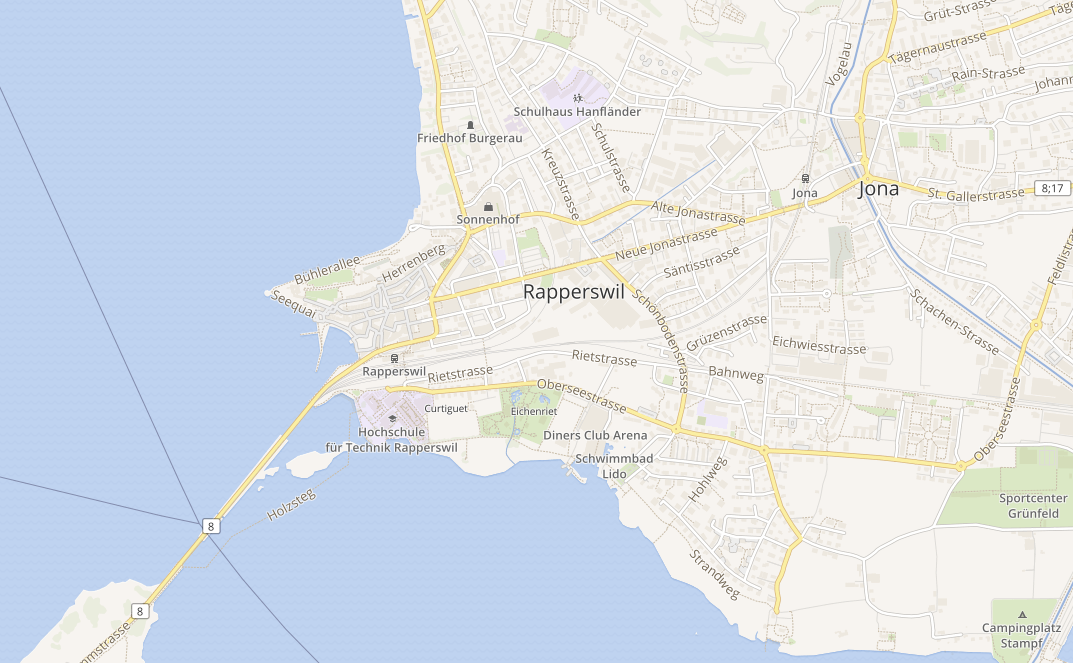
\includegraphics[width=1\textwidth]{images/unmodified_osm_bright.png}
  \caption{Unmodified OSM Bright visual style using osm2vectortiles}
\end{figure}

\section{Future}\label{part1_future}
In a first step the project should be expanded to provide vector tiles for the entire world. The vector tile rendering workflow needs to be scaled out for the entire world. Regular updates for the vector tiles have been requested by the members of the Swiss OSM community
and will require identifying and rerendering updated tiles.\\
The long-term vision of this project is to provide a complete offline map experience, including basic geographic name search. These suggestions will be the project goals for the bachelor thesis. More detailed listing of
future features can be found in \autoref{part2_results_and_future}.

\chapter{State of Technology}

As of today most web maps are based on raster tiles except a few big providers like Google, Mapbox and Apple.
%\marginpar{The \hyperref[history-of-webmaps]{\emph{History of Webmaps}} chapter provides more details.}
The rest of the industry is now in the transition from raster based maps into vector based maps. For vector based maps the Mapbox Vector Tile Specification\footnote{\url{https://github.com/mapbox/vector-tile-spec/tree/master/1.0.1}} is the most dominant Open Source specification of vector tiles.

\section{Current Vector Data Providers}

While the deployment setup for vector based maps is much simpler than
the traditional raster tile setup the most complex part is still
the creation of vector data which takes a lot of time and care.

\paragraph{Mapbox}

Mapbox provides vector tiles of the entire world as part of its
map hosting technologies since 2012 branded as Mapbox Streets\footnote{\url{https://www.mapbox.com/blog/announcing-mapbox-streets/}}. Mapbox also provides the vector data for buyers of their Mapbox Atlas Server\footnote{\url{https://www.mapbox.com/atlas/}} starting at \$49,000 and distributes quarterly updates for \$10,000 per year .

\paragraph{Mapzen}

Mapzen provides API access to their public vector tiles\footnote{\url{https://mapzen.com/projects/vector-tiles/}}.
%\marginpar{Mapzen vector tiles can also be requested in GeoJSON, TopoJSON and Open Science Map format.}
Mapzen states that access and the platform should remain free and Open Source\footnote{\url{https://mapzen.com/about/}}. Mapzen however
does not give access to the entire raw data and one is bound to
the limitations of the service.

\paragraph{Kartotherian}

The Kartotherian\footnote{\url{https://www.mediawiki.org/wiki/Maps}} project from the Wikimedia Foundation\footnote{\url{https://wikimediafoundation.org/wiki/}} is very similar to this project.
The goal is to provide a free Map service that everyone can use for free.
The process is documented but the data is still bound to the service and not available as download.
The quality of the vector tiles is continuously improved but still lacking very important features.
Kartotherian is a great project which we can contribute to with our improved map data.

\paragraph{Google and Apple}

Apple started using vector tiles in their Apple Maps product in 2012\cite{wiki:apple-maps}  and  Google is using vector tiles since 2013\cite{wiki:google-maps} but they are both not accessible for the general public and use a proprietary format. 

\section{Characteristics}

While the providers open the process they still own the data in order to keep their strategic advantages and promote the use of their products using this data.
The open process is a wonderful step in the right direction, yet it requires great understanding
of the technology and sufficient computing power to actually
execute the workflow of producing vector tiles with worldwide coverage.

\section{Shortcomings}

The providers already solve the problem of producing the vector tiles
and making it accessible. The data however can only be used
via their services.
\newline{}
Being able to download world data and use it in a custom server
infrastructure, offline and without strings attached is a big advantage
and a problem this thesis wants to solve.

\newpage
%------------------------------------------------
\part{Evaluation}
%------------------------------------------------

\part{Project Documentation}

\chapter{History of Webmaps}
\label{history-of-webmaps}

Web mapping has gone through different technologies and changes in
the recent years. It is important to understand the evolution of web maps to understand why vector tiles are quite a fundamental change in how maps work.

\paragraph{Phase 1: Untiled Static
Maps}

In the beginning WMS servers generated static images for an extract
of the map. Each view of a map requested a unique extract of a map that was generated for this person.


\paragraph{Phase 2: Raster Tiles}

In 2005 Google introduced Google Maps and XYZ 
tiles\footnote{\url{http://wiki.openstreetmap.org/wiki/Slippy_Map}}
which delivered a idempotent raster image for coordinates specified by a
tile index.


\paragraph{Phase 2.5: Raster Tiles with Vector
Overlays}

To provide a level of interactivity tools like
Leaflet\footnote{\url{http://leafletjs.com/}} support rendering vector
data like SVG on top of a raster base map.

In order to support fully interactive maps 

\paragraph{Phase 2.75: Raster Tiles from Vector
Tiles}

For backwards compatibility and faster serving of raster tiles vector
tiles where introduced to avoid querying a database.

\paragraph{Phase 3: Vector Tiles}

Vector tiles are delivered directly to the browser and rendered by Web
GL based clients.


Improving the use of vector data in web mapping is often shown as the next challenge
of web mapping \cite[p.~88]{gaffuri2012toward} 

\subsubsection{Vector Tile Formats}

\paragraph{Mapbox Vector Tiles}

When Mapbox introduced it's geography tool Mapbox Studio in 2013 they
created the \emph{Mapbox Vector Tiles Specification}
\footnote{\url{https://github.com/mapbox/vector-tile-spec}} which is
implemented by a variety of tools and clients
\footnote{\url{https://github.com/mapbox/awesome-vector-tiles}}
including \emph{Mapbox GL JS}, \emph{Open Layers 3}, \emph{Leaflet},
\emph{Mapzen Tangram} and Esri
\footnote{\url{https://www.mapbox.com/blog/vector-tile-adoption/}} in
the future.

\subsubsection{Geopackage}

The \emph{GeoPackage Encoding Standard} is the OGC counterpart to the
\emph{Mapbox Vector Tiles Specification} which was introduced later and
is supported by QGIS, ESRI and GDAL.

\subsubsection{Google Maps}

Google Maps is using vector tiles since 2010 under the hood and was the
first provider implementing this. Styling is limited and the format
propretiary.

\subsubsection{Mapbox}

In 2013 Mapbox introduced Mapbox Studio a geography tool working with
vector tiles.

\subsubsection{Mapzen}

Was machen andere / welche ähnlichen Arbeiten gibt es zum Thema? Was
kann von anderen verwendet werden?

\subsubsection{Vector Tile Providers}\label{vector-tile-providers}

\paragraph{Mapbox}

\paragraph{Kartotherian}

\paragraph{Mapzen}

Diese Einleitung soll für den Ingenieur irgendeiner Fachrichtung
verständlich sein.

Sie stellt die Aufgabe in einen grösseren Zusammenhang und liefert eine
genaue Beschreibung der Problemstellung.

Allfällige Vorarbeiten oder ähnlich gelagerte Arbeiten werden
diskutiert.

Theoretische Grundlagen sind nur so weit auszuarbeiten, als dies für die
Lösung der Aufgabe nötig ist (keine Lehrbücher schreiben).

Die Erkenntnisse aus den theoretischen Untersuchungen sind wenn immer
möglich direkt mit der Problemlösung zu verknüpfen.

%------------------------------------------------
%\part{Development Process}

%------------------------------------------------
%	THESIS CONTENT - APPENDICES
%------------------------------------------------
\appendix
\part{Appendix} % New part of the thesis for the appendix

%---------------------------------------
%	POST-CONTENT THESIS PAGES
%---------------------------------------
% Bibliography

\label{app:bibliography} % Reference the bibliography elsewhere with \autoref{app:bibliography}
\raggedright
\manualmark
\markboth{\spacedlowsmallcaps{\bibname}}{\spacedlowsmallcaps{\bibname}} 
\refstepcounter{dummy}

\addtocontents{toc}{\protect\vspace{\beforebibskip}} % Place the bibliography slightly below the rest of the document content in the table of contents
\addcontentsline{toc}{chapter}{\tocEntry{\bibname}}

\bibliographystyle{plainnat}
\bibliography{bibliography}
 % Bibliography
% Declaration

\refstepcounter{dummy}
\pdfbookmark[0]{Declaration}{declaration} % Bookmark name visible in a PDF viewer

\chapter*{Declaration} % Declaration section text

\thispagestyle{empty}

Hereby we acknowledge,

\begin{itemize}
		\item that we conducted this thesis by ourselves and without any external help,
			except with those, which are explicitly mentioned,
		\item that all used sources are cited academically correct, and 
		\item that I didn't use any copyright protected materials (e.g. images) in
			an unauthorized manner.
\end{itemize}

\bigskip
 
\noindent\textit{\myLocation, \myTime}

\bigskip

\begin{flushright}
    \begin{tabular}{m{8cm}}
    \hspace{1cm}
\includegraphics[width=.5\textwidth]{images/signature_lukas.jpg}
    \\ \hline
    \centering Lukas Martinelli, \today \\
    \end{tabular}
\end{flushright}

\begin{flushright}
    \begin{tabular}{m{8cm}}
    \hspace{2cm}
\includegraphics[width=.33\textwidth]{images/signature_manuel.png}
    \\ \hline
    \centering Manuel Roth, \today \\
    \end{tabular}
\end{flushright}


 % Declaration
%---------------------------------------

\end{document}
